Given is the periodic signal curve $s(t)$

\begin{figure}[H]
	\centering
	\begin{tikzpicture}
		\pgfplotsset{
			every axis plot/.append style={line width=1pt, mark=none}
		}
		\begin{axis}[
			clip=false,
			axis lines=middle,
			xmin=-0.5, xmax=12.5,
			xlabel={$t$},
			xmajorticks=false,
			ymin=-1.3, ymax=1.3,
			y=2.5cm,
			ylabel={$s(t)$},
			yticklabels={$\hat{s}$, $-\hat{s}$},
			ytick={1,-1},
			width=12cm,
			x label style={at={(current axis.right of origin)},	anchor=east, right=1mm},
			y label style={at={(current axis.above origin)}, anchor=south }
		]
			\addplot [samples=500, color=blue, domain=0:3.7*pi] {sin(deg(1.22*x))};
			
			% Nullstelle ist 0 + T*n / 2
			% T = 2*pi/1.22
			\draw[color=gray!80, line width=0.75pt, dashed] (2*pi/1.22, 0) -- (2*pi/1.22, 1.5);
			
			\draw[color=gray!80, line width=0.75pt, dashed] (2*pi/1.22/2*4, 0) -- (2*pi/1.22/2*4, 1.5);
			
			\draw[color=gray!80, line width=0.75pt, dashed] (2*pi/1.22/2*3, 0) -- (2*pi/1.22/2*3, 1.2);
			
			\draw[<->, color=gray!80, line width=0.75pt] (2*pi/1.22/2*2, 1.4) -- (2*pi/1.22/2*4, 1.4) node[midway, above] {\tiny $T_0$};
		\end{axis}
	\end{tikzpicture}
	\caption{\label{fig:416a}Characteristics of a periodic signal $s(t)$}
\end{figure}

\begin{enumerate}
	\item Rectified value(Gleichrichtwert) of the sinusoidal alternating voltage\newline
	In general, the rectification value(Gleichrichtwert) $\overline{\abs{s}}$ for a sinusoidal AC voltage describes an average value over the period duration that the signal generates after negative half-waves have been removed.
	\begin{equation*}
		\overline{\abs{s}} = \frac{1}{T_0}\int_{t_0}^{t_0+T_0}\abs{s(t)}\D{t}=\frac{1}{T_0}\int_{t_0}^{t_0+T_0}\abs{\hat{s}\cdot\sin\left(\omega_0\cdot{t}\right)}\D{t}
	\end{equation*}
	
	Calculation of the rectification value for $T_0=2\pi$, $\hat{s} = \mathrm{const.} = 1$
	\begin{figure}[H]
		\centering
		\begin{tikzpicture}
			\pgfplotsset{
				every axis plot/.append style={line width=1pt, mark=none}
			}
			\begin{axis}[
				clip=false,
				axis lines=middle,
				xmin=-0.5, xmax=12.5,
				xlabel={$t$},
				xmajorticks=false,
				ymin=-1.3, ymax=1.3,
				y=2.5cm,
				ylabel={$s(t)$},
				yticklabels={$\hat{s}$, $-\hat{s}$},
				ytick={1,-1},
				width=12cm,
				x label style={at={(current axis.right of origin)},	anchor=east, right=1mm},
				y label style={at={(current axis.above origin)}, anchor=south }
			]
				\addplot [name path=f1, samples=500, color=blue, domain=0:3.7*pi, restrict y to domain=0:1] {sin(deg(1.22*x))};
				\addplot [samples=500, color=blue!60, domain=0:3.7*pi, restrict y to domain=-1:0, dashed] {sin(deg(1.22*x))};
				\addplot [name path=f2, samples=500, color=blue, domain=0:3.7*pi, restrict y to domain=0:1] {sin(deg(1.22*x+pi))};
				
				\path[name path=axis] (axis cs:2*pi/1.22/2*2,0) -- (axis cs:2*pi/1.22/2*4,0);
				
				\addplot [thick, color=blue, fill=blue, fill opacity=0.05]
					fill between[of=f1 and axis, soft clip={domain=2*pi/1.22/2*2:2*pi/1.22/2*4}];
				\addplot [thick, color=blue, fill=blue, fill opacity=0.05]
					fill between[of=f2 and axis, soft clip={domain=2*pi/1.22/2*2:2*pi/1.22/2*4}];
				
				% Nullstelle ist 0 + T*n / 2
				% T = 2*pi/1.22
				\draw[color=gray!80, line width=0.75pt, dashed] (2*pi/1.22, 0) -- (2*pi/1.22, 1.5);
				
				\draw[color=gray!80, line width=0.75pt, dashed] (2*pi/1.22/2*4, 0) -- (2*pi/1.22/2*4, 1.5);
				
				\draw[color=gray!80, line width=0.75pt, dashed] (2*pi/1.22/2*3, 0) -- (2*pi/1.22/2*3, 1.2);
				
				\draw[<->, color=gray!80, line width=0.75pt] (2*pi/1.22/2*2, 1.4) -- (2*pi/1.22/2*4, 1.4) node[midway, above] {\tiny $T_0$};
			\end{axis}
		\end{tikzpicture}
		\caption{\label{fig:416b}Rectified signal $s_g(t)$ from figure ~\ref{fig:416a}, with integral areas}
	\end{figure}
	From figure ~\ref{fig:416b} it can be deduced that it is sufficient for the calculation to integrate over half a period and multiply this result by 2, as there are two positive half-waves in one period due to the rectification. This eliminates the amounts(Beträge) in the integral and the antiderivative(Stammfunktion) can be formed. Furthermore, the following generally applies to the circular frequency $\omega_0 = 2\pi/T_0.$
	{
		\setlength{\abovedisplayskip}{6pt}
		\setlength{\belowdisplayskip}{12pt}
		\begin{flalign*}
			\overline{\abs{s}} &= \frac{1}{T_0}\cdot2\int_{0}^{\frac{T_0}{2}}{s(t)}\D{t}
			=\frac{1}{T_0}\cdot2\int_{0}^{\frac{T_0}{2}}\hat{s}\cdot\sin\left(\omega_0\cdot{t}\right)\D{t}
			=\frac{2\hat{s}}{T_0}\int_{0}^{\frac{T_0}{2}}\sin\left(\omega_0\cdot{t}\right)\D{t} & \\
			& = \frac{2\hat{s}}{T_0}\cdot\left[\frac{-\cos\left(\omega_0\cdot{t}\right)}{\omega_0}\right]_0^{\frac{T_0}{2}}
			= \frac{\cancel{2}\hat{s}}{\bcancel{T_0}}\cdot\left[\frac{-\cos\left(\frac{2\pi}{T_0}t\right)}{\frac{\cancel{2}\pi}{\bcancel{T_0}}}\right]_0^{\frac{T_0}{2}} & \\
			& = \frac{\hat{s}}{\pi}\left(-\cos\left(\frac{\cancel{2}\pi}{\bcancel{T_0}}\cdot\frac{\bcancel{T_0}}{\cancel{2}}\right)+\cos\left(\frac{2\pi}{T_0}\cdot0\right)\right)
			= \frac{\hat{s}}{\pi} \left(-\cos\left(\pi\right)+\cos(0)\right) & \\
			& = \frac{2\hat{s}}{\pi} \approx \num{0,636}\overline{6}\;\hat{s}
		\end{flalign*}
	}
	\clearpage
	\item Description and representation of the curve and rectified value in Matlab
	\lstinputlisting[language=Matlab]{./assets/Lab1_416.m}
	{
		\setlength{\fboxsep}{0pt}%  
		\colorbox{backcolor}{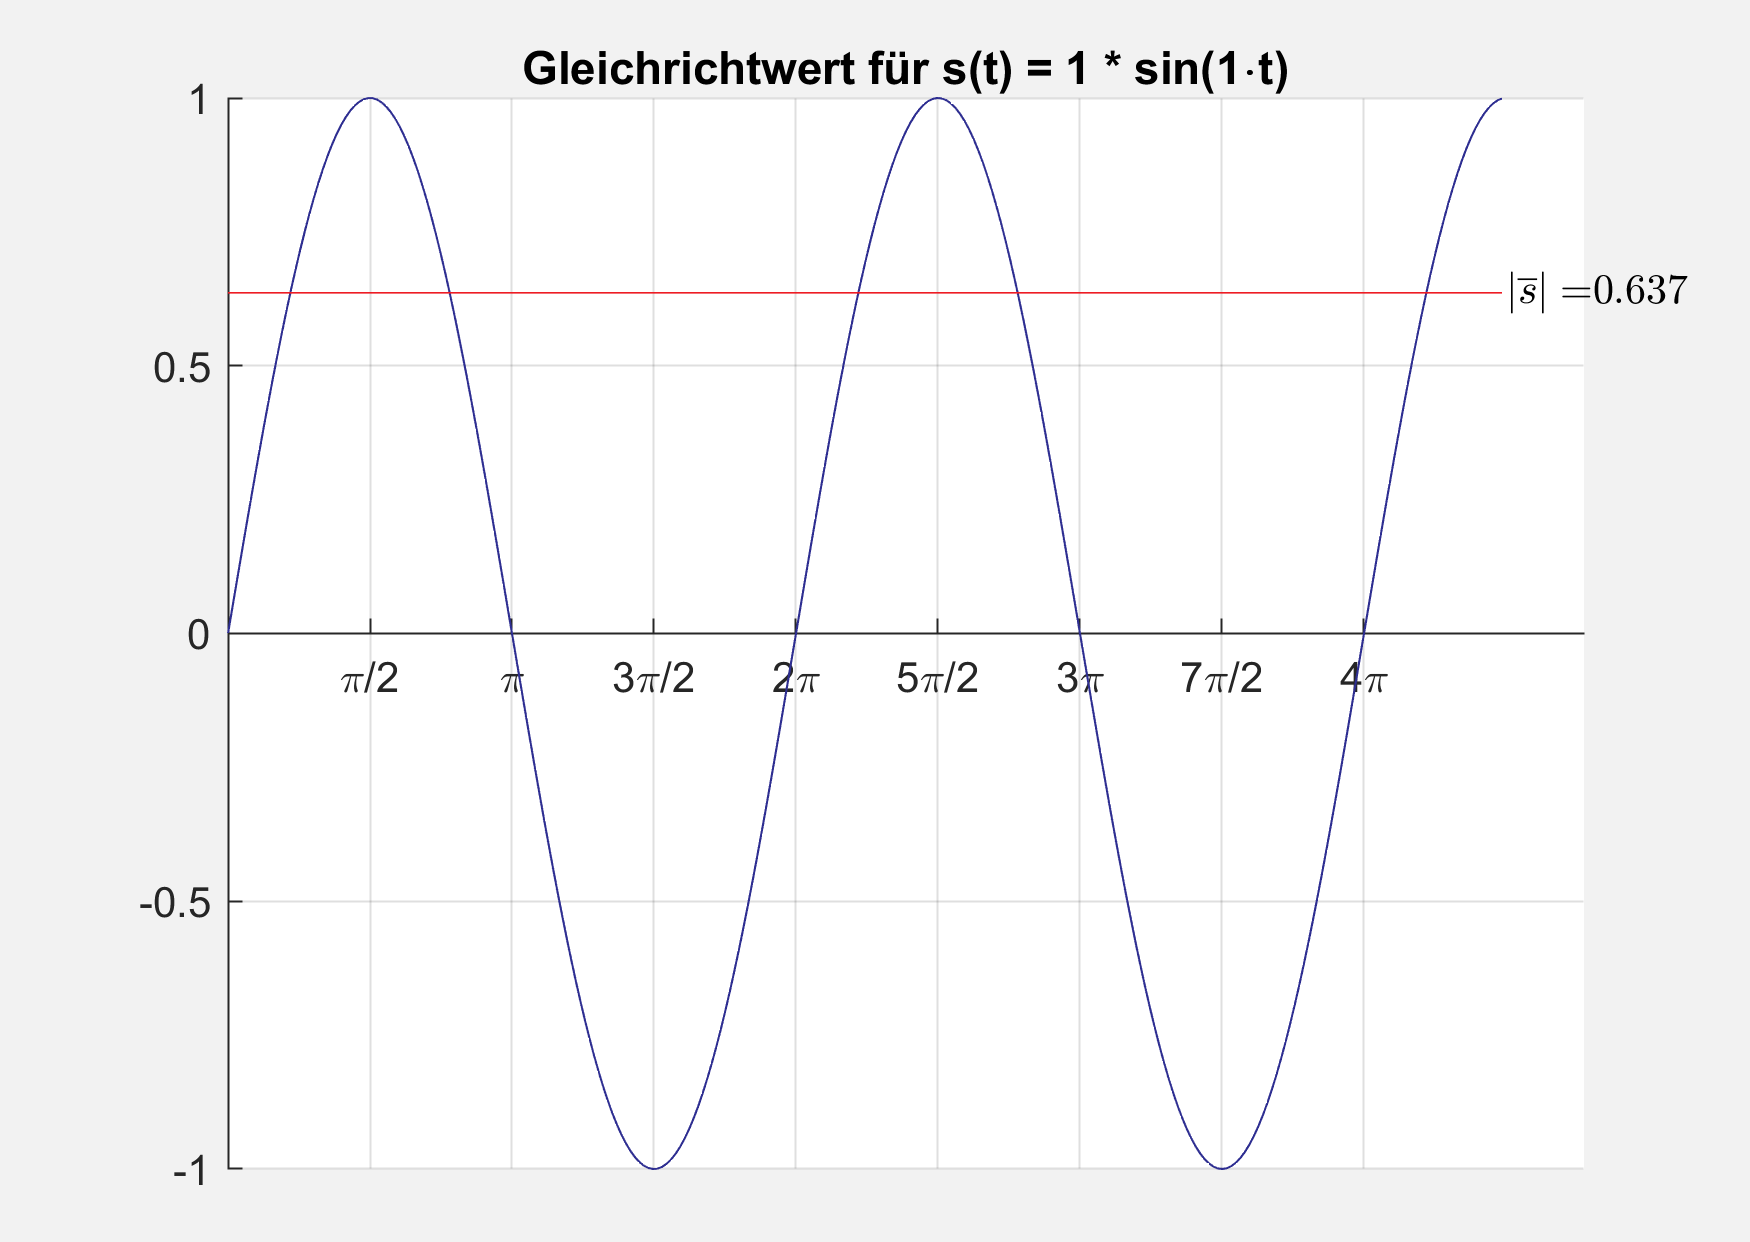
\includegraphics[width=\linewidth, keepaspectratio]{./assets/416.png}}
	}
\end{enumerate}